% 来源: 19c9fbbc-4a12-88c0-8000-00009d2ee8a0_4.3_包过滤.pdf
% 提取时间: 2026-02-28T22:51:36+08:00

4.3 包过滤
一种协议，就像复印中心或冰淇淋店一样，应该能够为多个客户端提供服务。协议的客户端可以是终端
用户（如文件传输协议的情况）、软件程序（例如，当traceroute工具使用互联网协议时），甚至是其他
协议（如电子邮件协议SMTP使用TCP的情况）。
因此，当一条消息到达时，接收协议必须将接收到的消息分发给适当的客户端。这个功能被称为解复
用。解复用是数据链路、路由和传输协议的一个组成部分。它是第2章抽象协议模型的基本部分。




\begin{figure}[htbp]
\centering
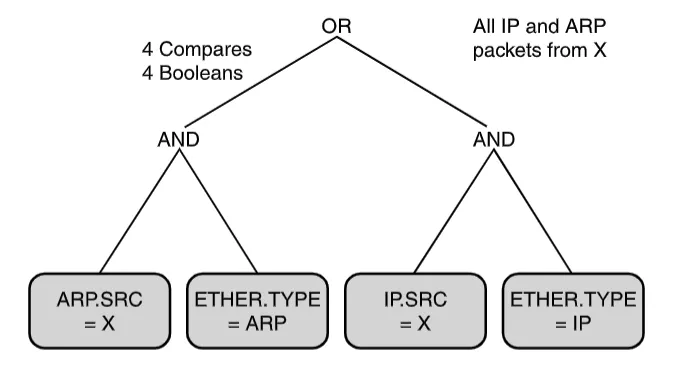
\includegraphics[width=0.8\textwidth]{../assets/ch04/ch04-4_3_包过滤-001.png}
\end{figure}
图8.1 传统的分层解复用是每一层利用层头部中的一个字段，将数据包解复用到上面的下一层软件。
传统上，解复用是通过使用接收到的消息各层头部中包含的解复用字段，逐层进行的。这种方式被称为
分层解复用，如图8.1所示。例如，在图中从下往上看，一个数据包可能通过以太网到达工作站。以太网
驱动程序会检查这个数据包，它会查看一个所谓的协议类型字段，以确定正在使用哪种路由协议（如
IP、IPX）。假设类型字段指定为IP，以太网驱动程序可能会向上调用IP软件。
在IP处理之后，IP软件会检查IP头部中的协议ID字段，以确定传输协议（如TCP或UDP？）。假设是
TCP，数据包将被传递给TCP软件。在完成TCP处理后，TCP软件会检查数据包中的端口号，以便将数
据包解复用到正确的客户端，例如，传递给实现HTTP的进程。
传统的解复用相当直接，因为每一层基本上都是对层头部中的某些字段进行精确匹配。这可以很容易地
实现，比如使用我们将在第10章描述的哈希方法。当然，每一层的查找成本会累积起来。
相比之下，本章重点讨论早期解复用，这在高速情况下是一项更具挑战性的任务。回顾图8.1，早期解复
用在数据包首次到达时，通过一次操作就能确定接收到的数据包所经过的整个协议路径。在最后一个例
子中，早期解复用可以一举确定网页数据包的路径是以太网、IP、TCP、网页。或许“分层解复用”是个
更好的术语。然而，本书采用了更被广泛接受的“早期解复用”这一名称。

                                                     1
一般来说，早期解复用的难点在于还需要允许应用程序灵活指定它们希望运行的底层协议，或者它们希
望接收其数据包的协议。这对于流量监测或安全应用特别有用。然而，如果早期解复用仅限于过去20年
已成为标准的TCP连接，那么问题就简单得多，并且（正如我们在第6章所示）可以通过数据包转向机制
来完成，该机制检查协议是否为TCP和IP（以太网中的类型字段），然后根据TCP四元组进行解复用。
回想一下，Linux通过两种方式之一进行“早期解复用”：要么使用TCP四元组的哈希值来分配负载（接收
数据包转向，即Receive Packet Steering或RPS），要么将数据包发送到运行应用程序的核心（接收流
转向，即Receive Flow Steering或RFS）。RFS也使用四元组的哈希值，但用它来索引一个表，表项指
向数据包应被转向的核心。
虽然这种基于简单哈希的机制在处理TCP和IP时效果很好，但它无法解决应用程序可以实时指定的其他协
议的早期解复用问题，例如流量监测应用所需的协议。这就是本章的主题。
本章的结构如下。8.1节阐述了早期解复用的原因，8.2节概述了高效解复用解决方案的目标。本章其余部
分研究了早期解复用的各种实现方式。本章从开创性的CMU/斯坦福数据包过滤器（CSPF）开始（8.3
节），接着介绍常用的伯克利数据包过滤器（BPF）（8.4节），最后介绍一些较新的方案，如
Pathfinder（8.5节）和DPF（8.6节）。
本章描述的解复用技术（以及所使用的相应原理）总结在表8.1中。
快速参考指南
伯克利数据包过滤器（BPF）是免费提供的。然而，其他解复用算法效率更高。希望设计解复用例程的
开发者应该考虑8.5节中描述的PathFinder。虽然动态数据包过滤器（DPF，见8.6节）速度更快，但许多
开发者可能会发现DPF中动态代码生成的需求是一个障碍。还要记得，对于TCP连接的早期解复用现在
已经成为标准，并且在Linux中可以通过各种转向机制实现。因此，本章中的技术仅对流量监测等灵活解
复用有用。
8.1 早期解复用的机遇与挑战
为什么早期解复用是个好主意呢？第6章讨论了以下基本动机。
 ● 灵活的用户级实现：早期解复用最初的原因是为了允许在用户级灵活实现协议，同时避免过多的上
   下文切换。
 ● 高效的用户级实现：随着时间的推移，开发者意识到早期解复用还可以通过最小化上下文切换次数
   来实现高效的用户级实现。主要的额外技巧是将协议实现构建为一个共享库，可以链接到应用程
   序。
请注意，随着针对TCP数据包的接收数据包转向原语的出现，如今在用户级实现TCP已经很容易。然
而，早期解复用还有其他优点。
 ● 数据包优先级排序：早期解复用允许对重要数据包进行优先级排序，并快速丢弃不必要的数据包。


                                                         2
   例如，第6章表明，通过对接收的数据包进行早期解复用，将数据包直接放入每个套接字队列中，可
   以缓解接收器活锁问题。这使得系统在过载时可以丢弃慢速进程的消息，同时允许表现良好的进程
   继续接收消息。更普遍地说，早期解复用对于通过服务区分来为流量流提供服务质量保证至关重
   要。如果所有流量都被解复用到一个公共的内核队列中，那么在过载期间共享缓冲区填满时，重要
   数据包可能会丢失。如今的路由器出于类似原因进行数据包分类（第12章和第14章）。早期解复用
   允许对数据流的处理进行显式调度；调度和计费可以结合起来，以防止诸如优先级反转等异常情
   况。
 ● 路径定制：一旦知道了数据包的路径，就可以对代码进行定制以处理该数据包，因为更广泛的上下
   文是已知的。例如，与其让每一层协议都检查数据包长度，不如本着P1原则只检查一次，避免明显
   的浪费。莫斯伯格（Mosberger）和彼得森（Peterson）在1996年将路径的理念发挥到了逻辑极
   致，他们描述了一种操作系统，其中路径是一等公民对象。
 ● 快速分发：本章和第6章已经通过数据包过滤器和用户级协议实现描述了这个想法的一个实例。早期
   解复用避免了每层的复用成本；更重要的是，它避免了有时在分层复用中可能产生的控制开销。
8.2 目标
如果早期解复用是个好主意，那么它容易实现吗？如果每个数据包在最外层（如数据链路层或网络层）
头部携带一些信息，用于标识最终端点，那么早期解复用就特别容易实现。这是P14原则的一个例子，即
在层头部传递信息。例如，如果网络协议是像ATM这样的虚电路协议，ATM虚电路标识符（VCI）可以
直接标识数据包的最终接收者。
然而，像IP这样的协议并没有提供这样的便利。多协议标签交换（MPLS）确实提供了这种便利，但正如
第11章所描述的，MPLS通常仅在路由器之间使用。即使使用像ATM这样的协议，可用的VCI数量也可能
有限。由于没有单个解复用字段，因此需要更复杂的数据结构，我们称之为数据包过滤器或数据包分类
器。当然，正如我们一开始所指出的，仅针对TCP连接使用TCP四元组的哈希值来实现这一点很容易，
但更通用的解决方案需要更好的数据结构。
这样的数据结构将完整的数据包头部作为输入，并将输入映射到一个端点或路径。直观地说，数据包的
端点代表接收应用程序进程，而路径代表在端点消耗数据包之前处理数据包时需要调用的协议序列。在
描述如何构建数据包过滤器之前，以下是一个好的早期解复用算法的目标。
 ● 安全性：许多早期解复用算法是在内核中基于用户级程序的输入实现的。每个用户程序P指定它希望
   接收的数据包。与Java程序一样，设计者必须确保不正确或恶意的用户不会影响其他用户。即使在
   今天，这对于流量监测也尤为重要。
 ● 速度：由于解复用是实时进行的，早期解复用代码应该快速运行，特别是在只指定了单个过滤器的
   情况下。
 ● 可组合性：如果N个用户程序指定了描述它们期望接收的数据包的数据包过滤器，理想情况下，实现
   应该将这N个单独的数据包过滤器组合成一个复合数据包过滤器。复合过滤器应该具有这样的特性：
                                                      3
  搜索复合过滤器比单独搜索N个过滤器中的每一个都要快，特别是对于较大的N。
本章从一个温和的生物学视角出发，描述了一系列数据包过滤器种类，每一种后续的改进都比前一种更
能实现这些目标。不出所料，最早的种类几乎已经“灭绝”，尽管它因其简单性和历史意义而值得关注。
8.3 CMU/斯坦福数据包过滤器：开创性的数据包过滤器
CMU/CSPF（莫古尔等人，1987年）是为了在Mach操作系统中实现用户级协议而开发的。在CSPF模型
中，应用程序向内核提供一个程序，描述它们希望接收的数据包。应用程序A提供的程序对数据包头部进
行操作，如果数据包应该被路由到应用程序A，则返回true。就像老款德州仪器计算器一样，这种编程语
言是一种基于栈的表达式树模型实现。




如\begin{figure}[htbp]
\centering
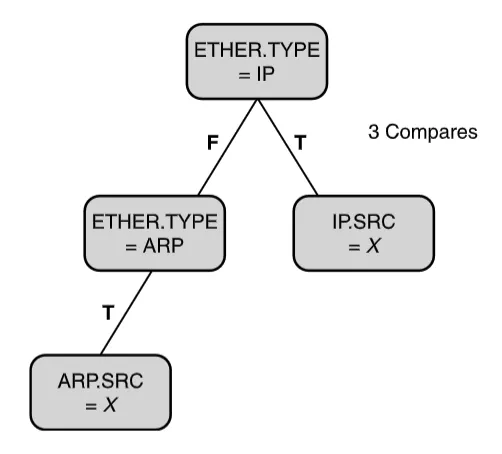
\includegraphics[width=0.8\textwidth]{../assets/ch04/ch04-4_3_包过滤-002.png}
\end{figure}
图8.2所示，树的叶子代表对数据包头部的简单测试谓词。一个测试谓词的例子是与固定值的相等比
较；例如，在图8.2中，ETHER.TYPE = ARP表示检查接收到的数据包中的以太网类型字段是否与为ARP
（地址解析协议）数据包指定的常量值匹配。树中的其他节点代表布尔运算，如AND和OR。
因此，图8.2中表达式树的左子树代表从源IP地址X发送的任何ARP数据包，而右子树代表从源IP地址X发
送的任何IP数据包。由于根节点代表一个OR操作，整个树表示请求由源X发送的所有IP或ARP数据包。这
样的表达式可以由调试工具代表希望检查来自源X的IP流量的用户提供给内核。

 图片加载失败
虽然表达式树模型提供了一种过滤器的声明性模型，但实际上这些过滤器使用一种命令式的基于栈的语
言来描述表达式树。为了确保安全性，CSPF提供了功能有限的栈指令；为了限制运行时间，它没有跳转
或循环结构。安全性还通过实时检查程序的加载和存储来实现，以消除非法的内存引用。因此，会监控
栈引用以确保其在栈范围内，并且会检查对数据包的引用以确保其在正在解复用的数据包长度范围内。
8.4 伯克利数据包过滤器：实现高性能监测

                                                      4
CSPF通过使用功能有限的指令和对内存访问进行运行时边界检查来保证安全性。然而，CSPF不具备可
组合性，并且在速度方面存在问题。数据包过滤器设计的下一个变革是引入了BPF（麦卡恩和雅各布
森，1993年）。
BPF的设计者特别希望将BPF用作高性能网络监测工具（如tcpdump）的基础，对于这些工具来说，速度
至关重要。他们注意到，即使使用如图8.2所示的单个CSPF表达式树，也存在两个速度问题。
 ● 架构不匹配：CSPF栈模型是为PDP - 11设计的，因此与现代RISC架构不太匹配。首先，必须模拟
   栈，这意味着每次进行布尔运算时都需要额外的内存引用来更新栈指针。其次，RISC架构通过将变
   量存储在快速寄存器中并直接从寄存器进行计算来提高效率。因此，为了在RISC架构中提高效率，
   尽可能多的计算应该在寄存器值被重用之前使用该寄存器值进行。例如，在图8.2中，CSPF模型每
   次引用以太网类型字段（检查与ARP和IP的相等性）时都将导致两次单独的内存加载。在现代机器
   上，更好的方法是将类型字段存储在寄存器中，并一次性完成所有与类型字段的比较，以减少内存
   引用。
 ● 模型效率低下：即使忽略CSPF所需的额外内存引用，表达式树模型通常也会导致比严格必要的操作
   更多。例如，在图8.2中，注意到CSPF表达式需要进行四次比较才能评估所有叶子节点。然而，注
   意到一旦我们知道以太网类型等于ARP（如果我们从左到右评估），那么额外检查IP源地址是否等于
   X就是多余的（原则P1，避免浪费）。主要问题是在表达式树模型中，随着计算的进行，没有办
   法“记住”数据包解析状态。这可以通过构建状态机的新模型来解决。
CSPF还有另外两个小问题。它只能解析数据包头部中固定偏移量处的字段；因此，它不能用于访问封装
在IP头部内的TCP头部，因为这需要首先解析IP头部长度字段。CSPF还仅使用16位字段处理头部，这使
得处理32位字段（如IP地址）所需的操作数量增加了一倍。
BPF通过以下方式解决了这些问题。首先，它用基于寄存器的语言取代了基于栈的语言，并带有一个间
接操作符，可以帮助解析TCP头部。使用“LOAD [12]”这样的命令将指定数据包偏移量处的字段加载到寄
存器中，该命令加载以太网类型字段，以太网类型字段恰好从以太网数据包的起始位置偏移12字节处开
始。
BPF然后可以进行比较和跳转，如“JUMP_IF_EQUAL ETHERTYPE_IP, TARGET1, TARGET2”。这条指
令将累加器寄存器与IP以太网类型字段进行比较；如果比较结果为真，程序跳转到行号TARGET1；否
则，跳转到TARGET2。BPF允许以8位、16位和32位块进行操作。




                                                                 5
更根本的是，BPF使用计算的控制流图（CFG）模型，如\begin{figure}[htbp]
\centering
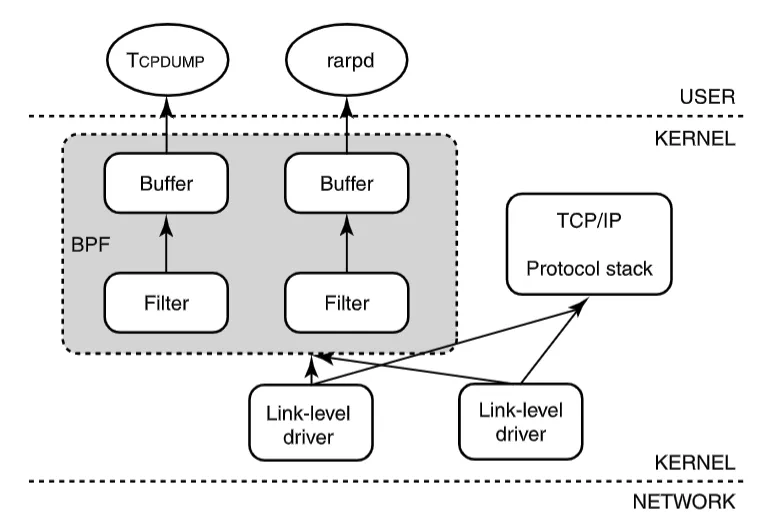
\includegraphics[width=0.8\textwidth]{../assets/ch04/ch04-4_3_包过滤-003.png}
\end{figure}
图8.3所示。这基本上是一个从根节点开始的状
态机，其状态在每个节点处更新，然后转移到其他节点状态，转移用指向其他节点的弧线表示。状态机
首先检查以太网类型字段是否为IP；如果是，则只需检查IP源字段是否为X即可返回true。如果不是，则
需要检查以太网类型字段是否为ARP以及ARP源是否为X。注意，在状态机的左分支中，我们不检查IP源
地址是否为X。因此，图8.3中最坏情况下的比较次数为3次，而图8.2中为4次。
BPF被用作许多工具的基础，包括著名的tcpdump工具，用户可以使用该工具获取链路上流动的TCP数
据包的可读记录。BPF被嵌入到BSD内核中，如\begin{figure}[htbp]
\centering
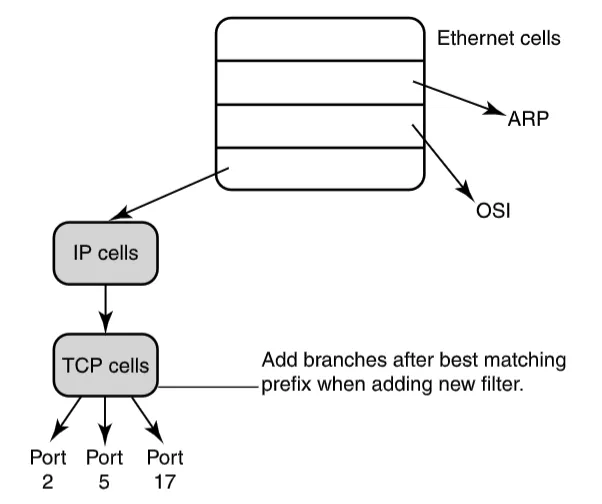
\includegraphics[width=0.8\textwidth]{../assets/ch04/ch04-4_3_包过滤-004.png}
\end{figure}
图8.4所示。




当数据包到达网络链路（如以太网）时，数据包由适当的链路层驱动程序处理，通常会传递到TCP/IP协
议栈进行处理。然而，如果BPF处于活动状态，则首先调用BPF。BPF根据当前指定的每个用户过滤器检
查数据包。对于每个匹配的过滤器，BPF将过滤器指定的尽可能多的字节复制到每个过滤器的缓冲区

                                                 6
中。注意，多个BPF应用程序可能会导致同一数据包的多个副本被缓冲。该图还显示了除tcpdump之外
的另一个常见BPF应用程序，反向ARP守护进程（rarpd）。
BPF还有两个对高性能也很重要的小特性。首先，BPF在缓冲之前过滤数据包，这避免了不必要的浪费
（P1），因为大多数接收到的数据包可能不是BPF应用程序想要的。这种浪费不仅包括缓冲区的内存，
还包括复制所需的时间（第5章）。
其次，由于数据包可能到达得非常快，而read()系统调用相当慢，BPF允许批处理（P2c），并允许在一
次调用中将多个数据包返回给监测应用程序。为了处理这个问题并区分数据包边界，BPF为每个数据包
添加一个头部，其中包括时间戳和长度。tcpdump的用户不必使用这个接口；相反，tcpdump提供了一
个更用户友好的接口：接口命令被编译为BPF指令。

 图片加载失败

8.5 Pathfinder：分解常见检查
BPF相较于CSPF是一种更优化的方案，因为它提高了单个过滤器的处理速度。然而，每个数据包仍必须
依次与每个过滤器进行比较。因此，处理时间会随着过滤器数量的增加而延长。幸运的是，对于典型的
BPF使用场景而言，这并非问题。例如，一个典型的tcpdump应用程序可能仅向BPF提供少量过滤器。
然而，在早期解复用用于区分大量数据包流或路径的情况下，情况就有所不同了。特别是，每个TCP连
接可能会提供一个过滤器，而繁忙服务器中的并发TCP连接数量可能非常大。为了应对这种环境变化
（用户级网络），出现了另一种成功的改进方案——Pathfinder（Bailey等人，1994年）。Pathfinder超
越了BPF，它具备可组合性，这使得它能够扩展以服务大量用户。
为了理解Pathfinder的解决方案，假设有500个过滤器，每个过滤器除了指定不同的TCP端口对外，其他
内容完全相同（以太网类型字段为IP，IP协议类型为TCP ）。如果依次处理每个过滤器，就需要将数据
包的以太网类型与（相同的）IP以太网类型字段进行500次比较，并将IP协议字段与（相同的）TCP协议
值进行500次比较。这显然是一种浪费（原则P1）。
接下来，将数据包中的TCP端口号与500个过滤器中每个指定的500个端口对进行比较，这种做法的弊端
并不明显。然而，这与线性搜索精确匹配的原理完全相同。这表明，当单个过滤器数量较多时，将所有
单个过滤器集成到一个复合过滤器中，可以显著减少不必要的比较。具体而言，可以使用哈希（原则
P15，使用高效的数据结构）来进行精确搜索，这样就可以用少量比较替代500次比较。
正如我们在本章开头反复提到的，如果仅处理TCP连接，这种哈希的概念已经通过接收数据包转向机制
实现。但如果想要对通用协议进行灵活的解复用，则需要更复杂的数据结构。
用于此目的的数据结构如图8.5所示。其基本思想是将BPF中每个过滤器的控制流图（CFG）进行叠加，
以便对同一字段的所有比较都放置在单个节点中。最后，每个节点都被实现为一个哈希表，其中包含所

                                                            7
有比较值，从而用哈希查找替代线性搜索。




 图片加载失败
图8.5展示了一个示例，其中至少有四个过滤器，其中两个指定目的端口号为2和5的TCP数据包；目前，
忽略指向TCP端口17的虚线，稍后将其作为过滤器插入的示例。除了TCP过滤器外，还有一个或多个指
定ARP数据包的过滤器，以及一个或多个指定使用OSI协议数据包的过滤器。
根节点对应以太网类型字段；哈希表包含过滤器中使用的每个可能的以太网类型字段值。每个节点条目
都有一个值和一个指针。因此，ARP条目指向进一步指定必须接收的ARP数据包类型的节点；OSI条目也
是如此。最后，对应IP的以太网类型字段指向对应IP协议字段的节点。
在IP协议字段节点中，对应TCP（值为6）的一个值将指向TCP节点。在TCP节点中，有三个值分别指向
目的端口值为2和5的过滤器（请记住，17尚未插入）。当一个TCP数据包到达时，解复用过程如下。
从根节点开始搜索，对以太网类型字段进行哈希处理，以找到与IP对应的匹配值。该值的指针将指向IP节
点，在IP节点中，对IP协议类型字段进行哈希处理，以找到与TCP对应的匹配值。该值的指针将指向TCP
节点，在TCP节点中，对数据包中的目的端口值进行哈希处理，以找到最终匹配的过滤器。
Pathfinder的数据结构与一种常见的数据结构——前缀树（trie）非常相似，第11章将更全面地介绍前缀
树。简而言之，前缀树是一种树结构，其中每个节点包含一个指向子树的指针数组；每个数组为固定字
符集中的每个可能值包含一个指针。
为了在前缀树中搜索关键字，需要将关键字分解为字符，并使用第i个字符对从根节点开始路径上的第i个
节点进行索引。以这种方式在节点i进行搜索会得到一个指针，该指针指向节点i + 1，然后在节点i + 1中
继续递归搜索。可以将Pathfinder结构视为对前缀树的扩展，它使用数据包头部字段（例如以太网类型字
段）作为连续的搜索字符，并使用哈希表替代每个节点中的数组。

                                                     8
众所周知，前缀树能够快速插入新的关键字。基于这种相似性，Pathfinder拥有快速插入或删除过滤器的
算法也就不足为奇了。例如，考虑插入一个对应TCP端口17的新过滤器。与前缀树一样，插入算法首先
搜索这个新过滤器的最长匹配前缀（第11章）。
这个最长匹配对应于路径“以太网类型 = IP，IP协议 = TCP”。由于此路径已由其他两个TCP过滤器创
建，因此无需重复创建。插入算法只需添加与新过滤器中超出最长匹配部分对应的分支（在这种情况下
是单个分支）。因此，只需更新TCP节点中的哈希表，添加一个指向端口17过滤器的新指针即可。
更准确地说，Pathfinder中的基本原子单元称为单元格（cell）。一个单元格指定数据包头部中的一个位
字段（使用偏移量、长度和掩码）、一个比较值和一个指针。例如，忽略指针，检查IP头部中协议字段
的单元格为(9, 1, 0xff, 6)——该单元格指定应将IP头部的第十个字节用全1掩码进行掩码处理，并与值6进
行比较，值6代表TCP。
给定用户的单元格串联在一起形成该用户的模式。多个模式通过不重新创建已存在的单元格进行叠加，
从而形成Pathfinder前缀树。最后，指定相同位字段但不同值的多个单元格使用哈希表进行合并。
除了使用哈希表替代数组外，Pathfinder还超越了前缀树，它使每个节点都包含任意代码。实际上，
Pathfinder认识到前缀树是一种特殊的状态机，可以通过在前缀树的每个节点执行任意操作来进行扩展。
例如，Pathfinder可以通过允许除前面描述的比较单元外的可加载单元来处理分片数据包。这是必要的，
因为对于分片数据包，只有第一个分片指定TCP头部；将各个分片链接在一起的是第一个分片中描述的
公共数据包ID。
Pathfinder通过在第一个分片到达后放置一个额外的可加载单元格（以及指定源地址等的正常IP比较单元
格）来处理分片，该可加载单元格加载数据包ID。通过不指定单元格中的比较值来指定一个单元格为可
加载单元格。
可加载单元格最初不是Pathfinder前缀树的一部分，而是IP单元格的一个属性。如果第一个分片匹配，则
将加载的单元格插入到Pathfinder前缀树中，现在它可以根据新加载的数据包ID匹配后续分片。在所有分
片都处理完毕后，可以删除这个新添加的单元格。最后，Pathfinder通过将后续分片的处理推迟到第一个
分片到达，来处理后续分片先于第一个分片到达的情况。
8.6 动态数据包过滤器：编译器来帮忙
到目前为止，Pathfinder被描述为一种树形结构，但实际上其数据结构可以泛化为有向无环图
（DAG）。有向无环图允许两个不同的过滤器在Pathfinder图中最初沿着不同的路径，然后汇聚到共享
的路径后缀。例如，在为目的端口80的TCP数据包提供过滤器时，该数据包可能是分片的，也可能是非
分片的，这种情况下有向无环图就很有用。虽然需要为分片和非分片的IP数据包分别指定不同的单元格
路径，但这两条路径可以指向同一组TCP单元格。
最后，Pathfinder还允许使用从单元格引出的“或”（OR）链接。其原理是，每个“或”链接指定一个值，
检查每个“或”链接以找到匹配的值，然后沿着该链接继续处理。

                                                        9
为了在拥塞期间对数据包进行优先级排序（如第6章所述），解复用例程必须在接收数据包所需的最短时
间内完成。Pathfinder的软件实现速度很快，但通常无法跟上线路速率。幸运的是，Pathfinder状态机可
以在硬件中实现，从而以线路速率运行。这与使用前缀树进行IP查找以线路速率工作的方式类似（第11
章）。
Bailey等人（1994年）描述的硬件原型为了提高速度牺牲了部分功能。它以16位块为单位工作，仅实现
了最基本的单元格功能；不过，它在硬件中实现了分片处理。功能的限制意味着Pathfinder硬件只能用作
缓存，以加速处理不太常见情况的Pathfinder软件。一个运行频率为100MHz的原型设计预计处理一个40
字节的TCP消息需要200纳秒，这对于1.5Gbps的速率来说已经足够。通过使用更快的时钟频率、更快的
内存和流水线遍历状态机，该设计可以扩展到更高的线路速率。
动态数据包过滤器：编译器来帮忙
Pathfinder的故事以借助硬件实现高速解复用作为结尾。鉴于如今大多数工作站和个人电脑不太可能配备
专用的解复用硬件，实现者似乎必须在早期解复用带来的灵活性和软件分类器有限的性能之间做出选
择。因此，高性能TCP（Clark等人，1989年）、主动消息（von Eicken等人，1992b）和远程过程调用
（RPC）（Thekkath等人，1993年）的实现都采用手工编写的解复用例程，也就不足为奇了。
动态数据包过滤器（DPF）（Engler和Kaashoek，1996年）试图同时兼顾灵活性和性能。DPF基于
Pathfinder前缀树的理念，但它通过在每次添加或删除过滤器时将分类器重编译为机器代码，消除了单元
格处理中固有的间接操作和额外检查。实际上，DPF为前缀树中的每个单元格生成单独的优化代码，而
不是使用可以解析前缀树中任意单元格的通用未优化代码。
DPF基于动态代码生成技术（Engler，1996年），该技术允许在运行时生成代码，而不是在内核编译时
生成。DPF应用了原则P2，即时间上的计算转移。需要注意的是，这里的运行时指的是分类器更新时
间，而不是数据包处理时间。
这一点很关键，因为这意味着DPF必须能够以足够快的速度重新编译代码，以免减慢分类器的更新速
度。例如，建立一个连接可能需要几毫秒，同时需要添加一个过滤器来识别端点。相比之下，以千兆速
率接收一个最小尺寸的数据包可能只需要几微秒。尽管有这样的时间差，但实现亚毫秒级的编译时间仍
然具有挑战性。
为了理解为何为每个单元格使用专门的代码是有用的，需要了解Pathfinder中单元格处理效率低下的两个
常见原因：
 ● 解释开销：Pathfinder代码在内核代码编译时确实会被编译为机器指令。然而，从某种意义上说，这
    些代码是在“解释”一个通用的Pathfinder单元格。例如，考虑一个指定了四元组（偏移量、长度、
    掩码、值）的通用Pathfinder单元格C。当数据包P到达时，用于检查单元格是否与数据包匹配的理
    想化机器代码如下：


                                                        10
 1                        将单元格中指定的偏移量加载到寄存器R1中 *)
     LOAD R1, C(Offset); (*
 2                        将单元格中指定的长度加载到寄存器R2中 *)
     LOAD R2, C(length); (*
 3                        将偏移量指定的数据包字段加载到R3中 *)
     LOAD R3, P(R1, R2); (*
 4                      将单元格中指定的掩码加载到寄存器R1中 *)
     LOAD R1, C(mask); (*
 5   AND R3, R1; (* 按照单元格中的指定对数据包字段进行掩码处理 *)
 6                       将单元格中指定的值加载到寄存器R2中 *)
     LOAD R2, C(value); (*
 7   BNE R2, R3; (* 如果掩码处理后的数据包字段不等于值，则进行分支 *)
请注意，第1、2、4和6行中的额外指令和额外内存引用是为了从通用单元格加载参数，以便后续进行比
较。
 ● 安全检查开销：由于用户编写的数据包过滤器不可信，所有实现都必须进行检查以防范错误。例
   如，必须在运行时检查对数据包字段的每次引用，以确保其在当前正在解复用的数据包范围内。同
   样，需要实时检查内存引用的对齐情况；在许多机器上，未对齐到字大小倍数的内存引用可能会导
   致陷阱。在进行这些额外检查后，前面显示的代码片段会变得更加复杂，并且包含更多指令。
通过为每个单元格专门编写代码，DPF可以利用将单元格添加到Pathfinder图时已知的信息，消除这两个
开销来源。
 ● 消除解释开销：由于DPF在创建单元格时就知道所有单元格参数，因此它可以生成将单元格参数直
   接编码为机器代码立即操作数的代码。例如，前面解析通用Pathfinder单元格的代码片段可以简化为
   更紧凑的特定单元格代码：
 1                             将数据包字段加载到R3中 *)
     LOAD R3, P(offset, length); (*
 2   AND R3, mask; (* 使用指令中的掩码对数据包字段进行掩码处理 *)
 3   BNE R3, value; (* 如果字段不等于值，则进行分支 *)
请注意，加载参数的额外指令以及（更重要的）额外内存引用已经消失，因为参数直接作为立即操作数
放置在指令中。
 ● 降低安全检查开销：在预期情况下（原则P11），可以通过在编译时推断大多数引用是字对齐的来减
   少对齐检查。这可以通过检查完整的过滤器来实现。如果初始引用是字对齐的，并且当前引用（偏
   移量加上所有先前头部的长度）是字长度的倍数，那么该引用就是字对齐的。只有在编译时推断失
   败时（例如，在进行间接加载时，如可变大小的IP头部），才需要进行实时对齐检查。同样，在编
   译时可以确定任何单元格中使用的最大偏移量，并在数据包处理之前进行一次检查，以确保最大偏
   移量在当前数据包的长度范围内。
一旦发现了好的方法，就应该充分利用它。DPF进一步利用编译时的知识进行如下优化。第一个优化是
将对相邻字段的小访问合并为一次大访问。其他优化将在练习中探讨。
DPF存在以下潜在缺点，但通过精心设计可以加以控制：
 ● 重新编译时间：回想一下，当向Pathfinder前缀树添加过滤器时（图8.5），只需创建原始前缀树中



                                                    11
   不存在的单元格。DPF通过缓存现有单元格的代码，并将这些代码直接复制（而不是从头重新创
   建）到新的分类器代码块中，对这种预期情况进行了优化（原则P11）。只有新创建的单元格才需要
   生成新代码。同样，当向哈希表添加新值时（例如，图8.5中添加的新TCP端口），除非哈希函数发
   生变化，否则代码将被重用，只需更新哈希表。
 ● 代码膨胀：解释的一个标准优点是代码更紧凑。为每个单元格生成专门的代码似乎会产生过多的代
   码，尤其是在过滤器数量较多的情况下。庞大的代码占用空间可能会反过来导致指令缓存性能下
   降。然而，仔细研究发现，DPF生成的不同代码块数量仅与所有过滤器检查的不同头部字段数量成
   比例。这比过滤器的数量更具扩展性。例如，对于10000个同时存在的TCP连接，DPF可能只生成三
   个专门的代码块：一个用于以太网头部，一个用于IP头部，以及一个用于TCP头部的哈希表。
DPF的最终性能数据令人印象深刻。在可比平台上，DPF解复用消息的速度比Pathfinder快13 - 26倍
（Engler和Kaashoek，1996年）。不过，添加过滤器的时间仅比Pathfinder慢三倍。动态代码生成只占
这种插入开销增加的40%。
无论如何，较大的插入成本似乎是为更快的解复用付出的合理代价。最后，DPF解复用例程似乎可以与
手工编写的解复用例程相媲美甚至超越它们；例如，一个用于解复用IP数据包的DPF例程只需要18条指
令，而Clark（1985年）报告的早期值为57条指令。虽然这两个实现是在不同的机器上进行的，但这些数
字在一定程度上体现了DPF的性能优势。
DPF带来的启示有两点。第一，DPF表明可以同时实现性能和灵活性。就像编译器生成的代码通常比手工
编写的代码更快一样，DPF代码似乎使手工编写解复用代码不再必要。第二，DPF表明以线路速率进行解
复用可能不需要硬件支持。实际上，在硬件实现中允许在创建过滤器时进行动态代码生成可能很困难。
软件解复用可以使用更便宜的工作站；它还可以使解复用代码从处理器速度的提升中受益。
技术变革可能使设计假设失效
在架构和操作系统领域，有不少创新在最初使用后被弃用，之后又重新被采用。这可能看起来像是时尚
的反复（比如“1995年褶边衣领又流行起来”），或者是重新发明轮子（即“天下并无新事” ），但要知道
何时以新的形式重拾旧想法，需要对当前技术有深入理解。
以电话网络核心为例，过去它通过模拟信号传输语音通话。随着光纤和晶体管的出现，如今电话网络核
心的大部分语音信号都采用T1和SONET层级体系进行数字传输。然而，随着光纤波分复用技术的出现，
至少有一些人讨论回归模拟传输。
因此，优秀的系统设计师必须持续关注现有技术，查看系统设计假设是否已不再成立。莫古尔等人在
1987年提出CSPF时提到了动态编译的概念，但并未深入探讨。CSPF的设计者认为，针对特定的过滤器
集定制代码（每次添加过滤器时都重新编译分类器代码）过于“复杂”。
在CSPF设计之时，动态编译可能速度较慢，而且无法在不同系统间移植；由于存在其他瓶颈，当时采用
动态编译所带来的收益也很有限。然而，到了设计DPF的时候，包括VCODE（恩格勒，1996年）在内的

                                                         12
许多系统已经设计出了相当快速且可移植的动态编译基础设施。DPF的其他分类器实现方式也消除了其
他瓶颈，这使得动态编译的优势更加明显。
8.7 结论
虽说“需求是发明之母”这句话略显陈词滥调，但它往往是正确的。新的需求推动新的创新；而没有需求
则解释了为什么创新没有更早出现。CSPF过滤器是在主要需求为避免进程上下文切换时实现的；在实现
这一目标后，提高过滤器性能就只是次要影响了。BPF是在主要需求为高效实现少数过滤器，以使像
tcpdump这样的监测工具能以接近线路速率运行时实现的。在实现这一目标后，扩展到大量过滤器的需
求似乎就没那么重要了。
Pathfinder是为了支持x - kernel（Hutchinson和Peterson，1991）中的用户级网络，并允许Scout
（Mosberger和Peterson，1996）将路径作为一等对象进行多方面利用而实现的。在找到了可行的硬件
实现方案后，或许提升软件性能就显得不那么重要了。DPF是为了在可扩展操作系统的环境中（Engler等
人，1995），实现高性能网络以及完全的应用级灵活性而设计的。表8.1总结了本章所使用的技术以及相
关的主要原理。
然而，鉴于如今TCP/IP的广泛应用，以及主流操作系统中数据包转向机制的可用性，目前还不清楚
Pathfinder和DPF在今天是否值得采用，毕竟它们增加了复杂性。BPF对于监测工具而言仍然有用。




                                                                 13
